\documentclass[aspectratio=169]{beamer}
\usetheme{SimplePlus}

\usepackage{tikz}
\usepackage{pgfplots}
\pgfplotsset{compat=1.17}
\usepackage{mathtools}
\usepackage{amsmath, amssymb, amsthm, bm}
\DeclareMathOperator{\grad}{\nabla}
\renewcommand{\P}{\mathbb{P}}
\newcommand{\R}{\mathbb{R}}
\newcommand{\ttag}[1]{(#1)}

\title[Finite Elements I]{Finite Elements Theory}
\author{Nicol\'as A. Barnafi}
\date{}

\begin{document}

\begin{frame}
    \titlepage
\end{frame}

\section{The Formalism}

\begin{frame}{The Finite Element Triple}
    \textbf{Definition (Ciarlet):} A Finite Element is a triple $(K, \mathcal{P}, \Sigma)$ where:
    \begin{itemize}
        \item $K \subset \mathbb{R}^d$ is the geometric domain (element).
        \item $\mathcal{P}$ is a finite-dimensional space of functions on $K$.
        \item $\Sigma = \{ \ell_1, \ell_2, \dots, \ell_n \}$ is a basis for $\mathcal{P}'$ (Degrees of Freedom).
    \end{itemize}

    \vspace{0.2cm}
    \begin{block}{Theorem}
        \textbf{Linear 1D FE is a Finite Element.}

        Let $K = [0, 1]$, $\mathcal{P} = \mathbb{P}_1(K)$, and $\Sigma = \{ \ell_1(v)=v(0), \ell_2(v)=v(1) \}$. \qed
    \end{block}
\end{frame}

\section{1D Higher Order}

\begin{frame}{Quadratic Elements ($\mathbb{P}_2$ in 1D)}
    \begin{columns}
        \begin{column}{0.6\textwidth}
            \textbf{Triple:}
            \begin{itemize}
                \item $K = [-1,1]$, with midpoint $0$.
                \item $\mathcal{P} = \mathbb{P}_2(K) = \text{span}\{\frac 1 2\xi(\xi-1),1-\xi^2, \frac 1 2 \xi(\xi+1)\}$.
                \item $\Sigma = \{ v(x_0), v(x_1), v(x_2) \}$.
            \end{itemize}
            \textbf{Unisolvence:} A polynomial of degree 2 with 3 roots is identically zero.
            
            \vspace{0.3cm}
            \textbf{Properties:}
            \begin{itemize}
                \item Interpolant $\Pi_h u$ is $C^0$-conforming.
                \item Convergence in $L^2$: $O(h^3)$.
                \item Convergence in $H^1$: $O(h^2)$.
            \end{itemize}
        \end{column}
        \begin{column}{0.39\textwidth}
            \begin{center}
            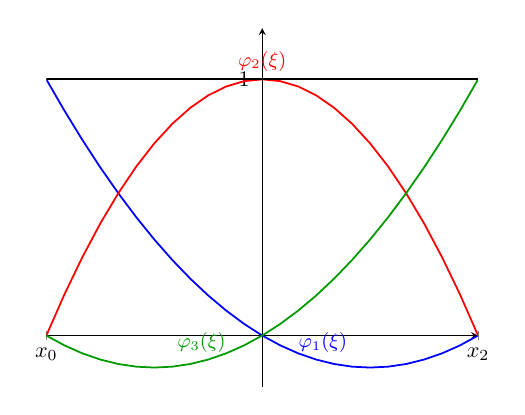
\begin{tikzpicture}[scale=0.8]
                \begin{axis}[axis lines=middle, ymin=-0.2, ymax=1.2, xtick={-1,0,1}, xticklabels={$x_0$,$x_1$,$x_2$}, ytick={1}]
                    \addplot[blue, thick, domain=-1:1] {0.5*x*(x-1)} node[blue, pos=0.7, anchor=south, font=\small] {$\varphi_1(\xi)$};
                    \addplot[red, thick, domain=-1:1] {1-x^2}node[red, pos=0.5, anchor=south, font=\small] {$\varphi_2(\xi)$};
                    \addplot[green!60!black, thick, domain=-1:1] {0.5*x*(x+1)}node[green!60!black, pos=0.3, anchor=south, font=\small] {$\varphi_3(\xi)$};
                    \addplot[black, thick, domain=-1:1] {1};
                \end{axis}
            \end{tikzpicture}
            \end{center}
        \end{column}
    \end{columns}
\end{frame}

\section{2D Elements}

\begin{frame}{2D Lagrange Elements: The Simplicial Triangle ($P_1$)}
    \begin{columns}
        \begin{column}{0.45\textwidth}
            \textbf{Triple $(K, \mathcal{P}, \Sigma)$:}
            \begin{itemize}
                \item $K$: Unit triangle $(0,0), (1,0), (0,1)$.
                \item $\mathcal{P} = \text{span}\{1, x, y\}$.
                \item $\Sigma = \{ v(x_i) \}_{i=1}^3$ (Nodal values).
            \end{itemize}
            \textbf{Basis Functions:}
            \begin{align*}
                \phi_1 &= 1 - x - y \\
                \phi_2 &= x \\
                \phi_3 &= y
            \end{align*}
        \end{column}
        \begin{column}{0.55\textwidth}
            \begin{center}
            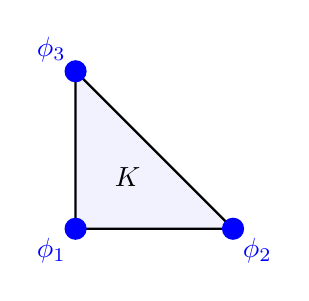
\begin{tikzpicture}[scale=2]
                \draw[thick, fill=blue!5] (0,0) -- (1,0) -- (0,1) -- cycle;
                \fill[blue] (0,0) circle (2pt) node[below left] {$\phi_1$};
                \fill[blue] (1,0) circle (2pt) node[below right] {$\phi_2$};
                \fill[blue] (0,1) circle (2pt) node[above left] {$\phi_3$};
                \node at (0.33, 0.33) {$K$};
            \end{tikzpicture}
            \end{center}
            \textbf{Conformity:} $V_h \subset H^1(\Omega)$ \\
            (Continuous across element interfaces).
            \textbf{Convergence Rates:}
            \begin{itemize}
                \item $L^2$ error: $O(h^2)$
                \item $H^1$ error: $O(h)$
            \end{itemize}

        \end{column}
    \end{columns}
\end{frame}

\begin{frame}{2D Lagrange Elements: The Quadrilateral Square ($Q_1$)}
    \begin{columns}
        \begin{column}{0.45\textwidth}
            \textbf{Triple $(K, \mathcal{P}, \Sigma)$:}
            \begin{itemize}
                \item $K$: Unit square $[0, 1]^2$.
                \item $\mathcal{P} = \text{span}\{1, x, y, xy\}$.
                \item $\Sigma = \{ v(x_i) \}_{i=1}^4$ (Nodal values).
            \end{itemize}
            \textbf{Basis Functions:}
            \begin{align*}
                \phi_1 &= (1-x)(1-y) \\
                \phi_2 &= x(1-y) \\
                \phi_3 &= xy \\
                \phi_4 &= (1-x)y
            \end{align*}
        \end{column}
        \begin{column}{0.55\textwidth}
            \begin{center}
            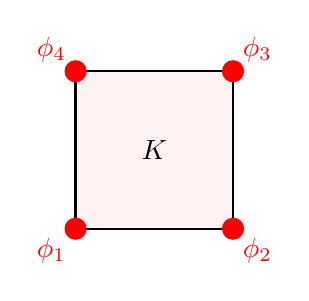
\begin{tikzpicture}[scale=2]
                \draw[thick, fill=red!5] (0,0) rectangle (1,1);
                \fill[red] (0,0) circle (2pt) node[below left] {$\phi_1$};
                \fill[red] (1,0) circle (2pt) node[below right] {$\phi_2$};
                \fill[red] (1,1) circle (2pt) node[above right] {$\phi_3$};
                \fill[red] (0,1) circle (2pt) node[above left] {$\phi_4$};
                \node at (0.5, 0.5) {$K$};
            \end{tikzpicture}
            \end{center}
            \textbf{Conformity:} $V_h \subset H^1(\Omega)$ \\
            (Bilinear interpolation ensures $C^0$).
            \textbf{Convergence Rates:}
            \begin{itemize}
                \item $L^2$ error: $O(h^2)$
                \item $H^1$ error: $O(h)$
            \end{itemize}

        \end{column}
    \end{columns}
\end{frame}

\section{Vector-Valued Elements}

\begin{frame}{Raviart-Thomas ($RT_0$) for $H(\text{div})$}
    \begin{columns}
        \begin{column}{0.5\textwidth}
            \textbf{Canonical Problem:} Mixed Poisson, Darcy flow.
            \begin{itemize}
                \item $\mathcal{P} = (P_0)^2 \oplus \bm{x} P_0$.
                \item $\Sigma = \{ \int_{e_i} \bm{v} \cdot \bm{n} \, ds \}_{i=1}^3$.
            \end{itemize}
            
            \vspace{0.2cm}
            \textbf{Unisolvence:} $\text{div} \bm{v} \in P_0$ and $\int \text{div} \bm{v} = \sum \int \bm{v} \cdot \bm{n}$.
        \end{column}
        \begin{column}{0.5\textwidth}
            \begin{center}
            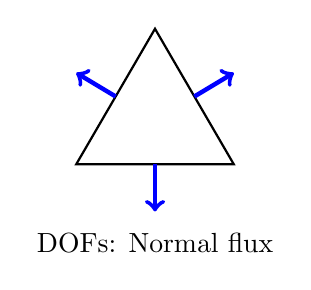
\begin{tikzpicture}[scale=2]
                \draw[thick] (0,0) -- (1,0) -- (0.5,0.86) -- cycle;
                \draw[->, ultra thick, blue] (0.5,0) -- (0.5,-0.3);
                \draw[->, ultra thick, blue] (0.75,0.43) -- (1.0,0.58);
                \draw[->, ultra thick, blue] (0.25,0.43) -- (0.0,0.58);
                \node at (0.5, -0.5) {DOFs: Normal flux};
            \end{tikzpicture}
            \end{center}
            \textbf{Conformity:} $H(\text{div}; \Omega)$.

            \textbf{Convergence Rate:} $H(\text{div};\Omega)$ error: $O(h)$
        \end{column}
    \end{columns}
\end{frame}

\begin{frame}{Why Normal Fluxes? Motivation for $RT_0$}
    \textbf{Problems:} For Darcy flow or conservation laws, we need $\bm{u} \in H(\text{div}; \Omega)$.

    \vspace{0.2cm}

    \vspace{0.2cm}
    \textbf{The Duality:}
    \begin{itemize}
        \item By the Divergence Theorem: $\int_K \text{div} \bm{v} \, dx = \int_{\partial K} \bm{v} \cdot \bm{n} \, ds$.
        \item To control the divergence inside $K$, we must control the flux on the boundary.
    \end{itemize}

    \begin{center}
    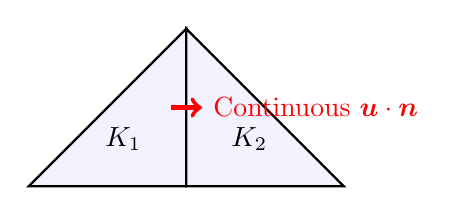
\begin{tikzpicture}[scale=2.0]
        \draw[thick, fill=blue!5] (0,0) -- (1,0) -- (1,1) -- cycle;
        \draw[thick, fill=blue!5] (1,0) -- (1,1) -- (2,0) -- cycle;
        \draw[ultra thick, red, ->] (0.9,0.5) -- (1.1,0.5) node[right] {Continuous $\bm{u} \cdot \bm{n}$};
        \node at (0.6, 0.3) {$K_1$}; \node at (1.4, 0.3) {$K_2$};
    \end{tikzpicture}
    \end{center}
    Nodal values are useless for $H(\text{div})$. We must define DoFs as \textbf{integral fluxes}.
\end{frame}

\begin{frame}{N\'ed\'elec ($N_0$) for $H(\text{curl})$}
    \begin{columns}
        \begin{column}{0.5\textwidth}
            \textbf{Canonical Problem:} Maxwell equations.
            \begin{itemize}
                \item $\mathcal{P} = (P_0)^2 \oplus \begin{pmatrix} -y \\ x \end{pmatrix} P_0$.
                \item $\Sigma = \{ \int_{e_i} \bm{v} \cdot \bm{t} \, ds \}_{i=1}^3$.
            \end{itemize}
        \end{column}
        \begin{column}{0.5\textwidth}
            \begin{center}
            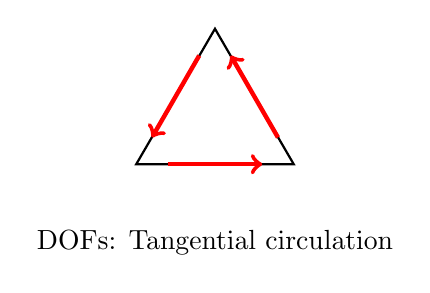
\begin{tikzpicture}[scale=2]
                \draw[thick] (0,0) -- (1,0) -- (0.5,0.86) -- cycle;
                \draw[->, ultra thick, red] (0.2,0) -- (0.8,0);
                \draw[->, ultra thick, red] (0.9,0.17) -- (0.6,0.69);
                \draw[->, ultra thick, red] (0.4,0.69) -- (0.1,0.17);
                \node at (0.5, -0.5) {DOFs: Tangential circulation};
            \end{tikzpicture}
            \end{center}

            \textbf{Conformity:} $H(\text{curl}; \Omega)$.

            \textbf{Convergence Rate:} $H(\text{curl};\Omega)$ error: $O(h)$
        \end{column}
    \end{columns}
\end{frame}

\begin{frame}{Why Tangential Circulation? Motivation for $N_0$}
    \textbf{Problems:} For Electromagnetics (Maxwell), we need $\bm{E} \in H(\text{curl}, \Omega)$.

    \vspace{0.2cm}
    \textbf{The Duality:}
    \begin{itemize}
        \item By Stokes' Theorem: $\int_S (\text{curl} \bm{v}) \cdot \bm{n} \, dS = \oint_{\partial S} \bm{v} \cdot \bm{\tau} \, dl$.
        \item To control the curl, we must control the circulation along edges.
    \end{itemize}

    \begin{center}
    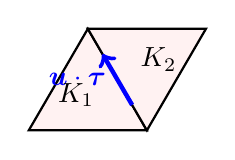
\begin{tikzpicture}[scale=1.5]
        \draw[thick, fill=red!5] (0,0) -- (1,0) -- (0.5,0.86) -- cycle;
        \draw[thick, fill=red!5] (0.5,0.86) -- (1,0) -- (1.5,0.86) -- cycle;
        \draw[ultra thick, blue, ->] (0.875, 0.215) -- (0.625, 0.645) node[midway, left] {$\bm{u} \cdot \bm{\tau}$};
        \node at (0.4, 0.3) {$K_1$}; \node at (1.1, 0.6) {$K_2$};
    \end{tikzpicture}
    \end{center}
    \textbf{Conclusion:} We assign DOFs to the \textbf{edge moments} of the mesh.
\end{frame}

\section{The Big Picture}

\begin{frame}{The Discrete De Rham Complex and Commutativity}
    These families ($\mathbb{P}, \mathbb{ND}, \mathbb{RT}$) is that they form a discrete complex that mimics the continuous one. The interpolation operators connect both worlds.

    \begin{center}
    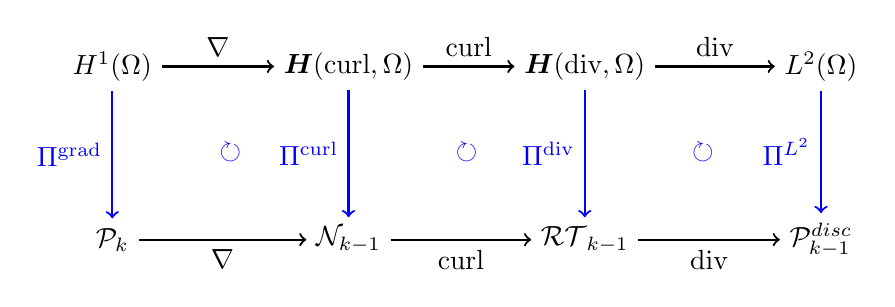
\begin{tikzpicture}[node distance=3cm, auto]
        % Continuous Spaces (Top Row)
        \node (H1) {$H^1(\Omega)$};
        \node (Hcurl) [right of=H1] {$\bm{H}(\text{curl}, \Omega)$};
        \node (Hdiv) [right of=Hcurl] {$\bm{H}(\text{div}, \Omega)$};
        \node (L2) [right of=Hdiv] {$L^2(\Omega)$};

        % Discrete Spaces (Bottom Row)
        \node (V1) [below of=H1, node distance=2.2cm] {$\mathcal{P}_k$};
        \node (V2) [below of=Hcurl, node distance=2.2cm] {$\mathcal{N}_{k-1}$};
        \node (V3) [below of=Hdiv, node distance=2.2cm] {$\mathcal{RT}_{k-1}$};
        \node (V4) [below of=L2, node distance=2.2cm] {$\mathcal{P}_{k-1}^{disc}$};

        % Continuous Operators
        \draw[->, thick] (H1) -- node {$\nabla$} (Hcurl);
        \draw[->, thick] (Hcurl) -- node {$\text{curl}$} (Hdiv);
        \draw[->, thick] (Hdiv) -- node {$\text{div}$} (L2);

        % Discrete Operators
        \draw[->, thick] (V1) -- node[below] {$\nabla$} (V2);
        \draw[->, thick] (V2) -- node[below] {$\text{curl}$} (V3);
        \draw[->, thick] (V3) -- node[below] {$\text{div}$} (V4);

        % Interpolation Operators (Vertical)
        \draw[->, thick, blue] (H1) -- node[left] {$\Pi^{\text{grad}}$} (V1);
        \draw[->, thick, blue] (Hcurl) -- node[left] {$\Pi^{\text{curl}}$} (V2);
        \draw[->, thick, blue] (Hdiv) -- node[left] {$\Pi^{\text{div}}$} (V3);
        \draw[->, thick, blue] (L2) -- node[left] {$\Pi^{L^2}$} (V4);

        % Commuting Symbols
        \node[blue] at (1.5, -1.1) {$\circlearrowright$};
        \node[blue] at (4.5, -1.1) {$\circlearrowright$};
        \node[blue] at (7.5, -1.1) {$\circlearrowright$};
    \end{tikzpicture}
    \end{center}

    \textbf{The Commuting Diagram Property:}
    $$ \text{curl}(\Pi^{\text{curl}} \bm{v}) = \Pi^{\text{div}}(\text{curl} \bm{v}) \quad \forall \bm{v} \in \bm{H}(\text{curl}, \Omega) $$
    This guarantees that the discrete operators preserve the exact kernels.
\end{frame}

\end{document}
